    Le but de ce chapitre est d'étudier formellement divers ensembles de chaînes de caractère ayant de ayant des propriétés intéressantes du point de vue informatique.
    
    \chaptertoc
    
    \section{Langages réguliers}
    
    \subsection{Alphabets, mots et langages}
    
    La première composante essentielle à un langage est son alphabet. On a une compréhension assez intuitive de ce concept, ne serait-ce qu'en pensant à l'alphabet latin, l'alphabet grec, l'alphabet cyrillique, \dots On voit donc un \guill{alphabet} comme un \textit{ensemble} de différents \textit{symboles}, qu'on appelle aussi souvent \textit{lettres}. En informatique, on reprend cette notion, en la définissant ainsi :
        
    \begin{definition}{Alphabet, lettres}{}
        On appelle \hg{alphabet} un \hg{ensemble non vide et fini}. On appelle \hg{lettres} ou \hg{symboles} les éléments de cet ensemble.
    \end{definition}
    %
    \begin{notation}
        On désignera usuellement par \hg{$\Sigma$ un alphabet}, et par \hg{$a, b, c, \dots$ les lettres} de $\Sigma$.
    \end{notation}
    
    On donne ci-dessous quelques exemples d'alphabets utilisés en informatique :
    
    \begin{example}{}{}
        \begin{enumerate}
            \itt On a \hg{$\Sigma = \ens{0, 1}$} l'\textit{alphabet} des \hg{nombres en binaire}.
            
            \itt On a $\hg{\Sigma = \ens{a, b, c, \dots, z}}$ l'\textit{alphabet} \hg{latin} (ici constitué des \textit{lettres} minuscules non accentuées).
            
            \itt On a l'\textit{alphabet} des \hg{caractères \texttt{Unicode}}.
        \end{enumerate}
    \end{example}
    
    Une fois les notions d'alphabet et de lettre introduites, on peut considérer la notion de mot, qu'on peut voir comme une suite finie de lettres d'un alphabet :
    
    \begin{definition}{Mot, longueur}{}
        Soit \hg{$\Sigma$} un \hg{alphabet} et \hg{$n \in \bdN$} un \hg{entier naturel}.
        %
        \begin{enumerate}
            \itast On appelle \hg{mot} (sur $\Sigma$) un \hg{$n$-uplet $u \in \Sigma^n$}.
            
            \itast On appelle \hg{longueur} du mot \hg{$u \in \Sigma^n$} l'\hg{entier $n$}.
            
            \itast On appelle \hg{mot vide} l'unique mot \hg{$\emptyset \in \Sigma^0$} de \hg{longueur nulle}.
        \end{enumerate}
    \end{definition}
    
    \begin{notation}
        \begin{enumerate}
            \itt On utilise usuellement \hg{$u$}, \hg{$v$}, \hg{$w$}, \hg{$x$}, \hg{$y$} et \hg{$z$} pour représenter un \hg{mot}.
            
            \itt L'\hg{ensemble des mots} sur $\Sigma$ est également noté \hg{$\Sigma^\star$}.
            
            \itt La \hg{longueur du mot $u \in \Sigma^\star$} est notée \hg{$\mod{u}$}.
            
            \itast Le \hg{mot vide} est généralement désigné par \hg{$\epsilon$}.
        \end{enumerate}
    \end{notation}
    
    On donne donc ci-dessous quelques exemples d'ensembles de mots :
    %
    \begin{example}{}{}
        \begin{enumerate}
            \itt Considérons l'\hg{alphabet $\Sigma = \ens{a, b, c}$}, on a l'\hg{ensemble des mots} de longueur inférieure ou égale à $2$ suivant :
            %
            \[ \hg{\ens{u \in \Sigma^\star \enstq \mod{u} \leq 2} = \ens{\epsilon, a, b, c, aa, ab, ac, ba, bb, bc, ca, cb, cc, aaa, \dots}} \]
            
            \itt Considérons un microprocesseur de \texttt{64 bits}. On a l'\hg{alphabet $\Sigma = \ens{0, 1}$}.
            
            L'ensemble des \hg{valeurs possibles pour un registre de calcul} est alors \hg{$\ens{\vphantom{\dfrac{}{}}u \in \Sigma^\star \enstq \mod{u} = 64}$}. 
        \end{enumerate}
    \end{example}
    
    On peut dès lors commencer à donner une structure aux notions précédemment définies. Une première opération usuelle est le fait de \guill{regrouper} deux mots, \ie la concaténation :
    
    \begin{definition}{Concaténation}{}
        Soit $u = a_1\dots a_n$ et $v = b_1\dots b_m$ deux mots sur $\Sigma$ de longeurs $n$ et $m$. On appelle \hg{concaténation} de $u$ et $v$ le mot $w = a_1\dots a_nb_1 \dots b_n$ de longueurs $n + m$. Ce mot est noté $uv$ (ou $u \cdot v$).
    \end{definition}{}{}  
    
    On remarquera que l'opération $\cdot$ de concaténation est une loi interne associative \textit{- on a bien $\p{uv}w = u\p{vw}$ -} de $\Sigma^\star$, dont $\epsilon$ est l'élément neutre. On dit que $(\Sigma^\star, \cdot)$ est un \textit{monoïde}.
    
    
    \begin{definition}{Puissance}{}
        Soit $\nu \in \Sigma^\star$ et $n \in \bdN$ :
        \begin{enumerate}
            \itt $\nu^0 = \epsilon$
            \itt $v^{n+1} = \nu \cdot \nu^n$
        \end{enumerate}
    \end{definition}
    
    \begin{example}{}{}
        $a^4b^2c^2 = a a a a b b c c$
    \end{example}
    
    \begin{definition}{Préfixe, suffixe}{}
        Soit $\p{u, v, w} \in (\Sigma^\star)^3$ tel que $w=uv$. On dit que :
        \begin{enumerate}
            \itt u est un \hg{préfixe de w}
            \itt v est un suffixe de w
        \end{enumerate}
    \end{definition}
    
    On remarque que tout mot non vide possède au moins 2 préfixes (ou suffixes) : $\epsilon$ et lui-même. $u = u\epsilon = \epsilon u$
    
    \begin{example}{}{}
        Les préfixes du mot $abbab$ sont : $\ens{\epsilon, a, ab, abb, abba, abbab}$.
    \end{example}
    
    \begin{definition}{facteur}{}
        Soit $w \in \Sigma^\star$.
        On dit que u est un facteur de w si :
        $\exists (v,v') \in (\Sigma^\star)^2$ tel que $w = v u v'$
        
    \end{definition}
    
    \begin{definition}{Sous-mot}{}
        Soit $w=a_1 \dots a_n$ un mot sur $\sigma$.
        Un \hg{sous-mot} est un mot de la forme $a_{i_1} \dots a_{i_k}$ avec $1 \leq i_1 < \dots < i_k \leq n$
        
    \end{definition}
    
    \begin{warning}{}{}
        Ne pas confondre "facteur" et "sous-mot".
        \begin{enumerate}
            \itt bca est un facteur de w.
        \end{enumerate}
    \end{warning}
    
    \begin{example}{}{}
        $w=abcabc$
        \begin{enumerate}
            \itt $bca$ a est un sous mot de $w$
            \itt $abab$ est un sous mot de $w$
            \itt $cac$ est un sous mot de $w$
            
            
        \end{enumerate}
        
        On remarque que les relations "être préfixe, suffixe, facteur, sous-mot" sont des \hg{relations bien fondées} sur $\sigma^\star$.
        
    \end{example}
    \begin{definition}{mot miroir}{}
        \begin{enumerate}
            \itt on appelle mot miroir de w et note $w^R$
        le mot $w^r =  a_1 \dots a_n$
            \itt un palindrome est un mot qu'on peut lire dans les deux sens tel que $w=w^R$
            
            
            
        \end{enumerate}
        
    \end{definition}
    
    \begin{definition}{Langage}{}
        Un langage $L$ sur un alphabet $\Sigma$ et un sous ensemble $\Sigma^*$ 
    \end{definition}
    
    \begin{example}{}{}
        On prend $\Sigma = \ens{a, b, c}$.
        %
        \begin{enumerate}
            \itt $L_1 = \ens{abc, bca, acb}$ est un langage fini.
            
            \itt $L_2 = \ens{ab^nc \enstq n \in \bdN}$ est le langage infini des mots commençant par $a$; suivi d'une suite (de taille arbitraire) de $b$, et finissant par $c$.
            
            \itt $L_3 = \ens{a^n \enstq n \in \bdP}$
        \end{enumerate}
    \end{example}
    
    \begin{notation}
        On note $\overline{L}$ le complémentaire de L :
        $\overline{L} = \Sigma^* \backslash L$
    \end{notation}
    
    \begin{definition}{Concaténation de deux langages}{}
        Soit $L_1 et L_2$ des langages sur $\Sigma$.
        Le langage \hg{concaténation}  de $L_1$ et $L_2$, noté $L_1 L_2$, est défini par :
        $L_1 L_2 = \ens{\omega \enstq \exists u \in L_1, \exists v \in L_2, \omega = uv}$
    \end{definition}
    
    \begin{example}{}{}
        $L_1 = \ens{aa, ab, bc} ; L_2 = \ens{\epsilon, a, abc}$
        $L_1 L_2 = \ens{aa, ab, bc, aaa, aba, bca, aaabc, ababc, bcabc}$
    \end{example}
    
    \begin{definition}{Puissance d'un language }
        Soit $L \subset \Sigma^*$, Soit $n\in \bcN$  
        
        
        Le langages $L^n$ est definit par récurrence sur $n$
        \begin{enumerate}{}{}
            
            \itt $L^0 = \ens{ \varepsilon}$
            
            \itt %lol itt comme un jour d'itt 
                $L^n+1 = L * L^n $ pour $n \geq 0$ 
                
        \end{enumerate}{}
        
    \end{definition}
    
    \begin{warning}{}{}
        \begin{enumerate}
            \itast Ne pas confondre $\emptyset$ et $\ens{\epsilon}$
            
            \itast Ne pas confondre $L^n$ et $\ens{u^n \enstq u \in L}$
        \end{enumerate}
    \end{warning}
    
    \begin{definition}{Étoile de Keeme}{}
        Soit \hg{$L \subset \Sigma^\star$}. On appelle \hg{étoile de \textsc{Kleene} de $L$} le langage \hg{$\displaystyle \bigcup U_{n \in \bdN} L^n$}.
    \end{definition}
    
    \begin{notation}
        L'\hg{étoile de \textsc{Kleene} de $L$} est généralement notée \hg{$L^\star$}.
    \end{notation}
    
    On remarque que
    \begin{enumerate}
        \itt c'est de la que vient la notation $\Sigma^\star$
        \itt On note parfois $L^+ = \bigcup_{n > 0} L^n$
    \end{enumerate}
    
    \begin{definition}{langage miroir}{}
        Soit $L \subset \Sigma^\star$. On appelle langage mirroir de L le langage $L^r$ défini par $L^r = \ens{\omega^r \enstq \omega \in L}$
        
    \end{definition}
    
    \subsection{Langage réguliers, expression régulières}
    
    \begin{definition}{Langage réguliers}{} 
        Soit $\Sigma$ un alphabet. L'ensemble des langages réguliers sur $\Sigma$ (ou langages rationnels sur $\Sigma$) est défini inductivement par: 
        \begin{enumerate}
            \itast $\emptyset$ est un langage régulier
            
            \itast  Pour tout $a \in \Sigma$, $\ens{a}$ est régulirer ;
            
            \itast si $A$ et $B$ sont des langages réguliers, alors $A \cup B$, $AB$ et $A^\star$ sont réguliers.
            
        \end{enumerate}
    \end{definition}
    %
    \begin{notation}
        On note $\Reg_\Sigma$ l'ensemble des langages réguliers sur $\Sigma$.
    \end{notation}
    
    Parfois, on inclut dans la définition précédente que $\ens{\epsilon}$ est régulier. Ceci est en fait redondant car $\ens{\epsilon} = \emptyset^\star$
    
    \begin{definition}{Expression régulière}{}
        
        Une expression régulière sur un alphabet $\Sigma$ ou expression rationnelle est définie inductivement 
        %
        \begin{enumerate}
            \itast $\emptyset$ et $\epsilon$ sont*µ des expressions régulières.
            
            \itast pour tout $e \in \Sigma$, $e$ est une expression régulière.
            
            \itt si $r_1 et r_2$ sont deux expression réguliere 
                \begin{enumerate}
                    \itt $r_1 | r_2$ est une expression réguliere 
                    
                    \itt $r_1, r_2$ est une expression régulière
                    
                    \itt $r_1^* $ est une expression régulière
                \end{enumerate}
        \end{enumerate}
    \end{definition}
    
    On notera que les règles de priorité sont ${}^\star > \cdot > \vert$.
    
    
    \begin{definition}{Langage d'une expression reguliere}{}
        Soit r une expression reguliere sur $\Sigma$
        
        le langage de l'equation r, noté $\bsL(r)$, est defini par induction structurelle sur r≠
        
        
        \begin{enumerate}
            \itt $\bsL\p{\emptyset} = \ens{\emptyset}$
            \itt $\bsL\p{\epsilon} = \ens{\epsilon}$
            \itt $\forall a \in \Sigma, \bsL\p{a} = \ens{a}$
            \itt $\bsL\p{r_1 \enstq r_2} = \bsL \p{r_1} \cup \bsL \p{r_2}$
            \itt $\bsL\p{r_1 r~……∞,_2} = \bsL \p{r_1} \bsL \p{r_2}$
            \itt $\bsL\p{r^\star} = \bsL \p{r}^\star$ 
        \end{enumerate}
    \end{definition}{}
    
    \begin{example}{}{}
        \begin{enumerate}
            \itt $mpi^\star : \ens{mpi \dots i}$
            \itt $\p{mpi}^\star : \ens{mpimpi \dots mpi}$
            
            \itt L'ensemble des nombres en base 2 sans zéro non significatif est reconnu par
            $0 \vert 1 \p{0 \vert 1}^\star$
            
            \itt $0^\star 1 0^\star 1 0^\star 1 0^\star$ décrit le langage des mots sur $\Sigma = \ens{0, 1}$ contenant exactement trois 1.
        
            \itt $\p{a \vert b \vert c \vert \dots \vert z \vert .\vert-}^\star @ \p{a \vert \dots \vert z \vert -}.\p{com \vert fr \vert \dots}$
            est l'ensemble des adresses mails syntaxiquement correctes.
        \end{enumerate}
    \end{example}
    
    \begin{enumerate}
        \itt En anglais, le terme \textit{regular expression} est souvent abrégé en \textit{regex}.
        
        \itt sous \textit{Linux}, l'outil \texttt{grep} permet de rechercher un motif dans des fichiers a l'aide d'expression régulières :
        %
        \[ \text{\sffamily\textbf Globally \textbf regular \textbf expression \textbf print }\]
        
        L'outil \texttt{grep} utilise une syntaxe étendue (\textsf{POSIX}) pour décrire les expressions régulières (\cf TP1).
        
    \end{enumerate}
    
    \section{Automates finis}
    
    Les automates sont des objets calculatoires fondamentaux a l'informatique.
    Il en existe de nombreusses variantes, selon le domaine d'application 
    \begin{enumerate}
        
        \itt automates finis 
        \itt automates à pile 
        \itt automates d'arbre 
        \itt automates àcompteurs 
        \itt automates temporisés 
        
    \end{enumerate}
    
    Voici quelque applications
    
    \begin{enumerate}
        \itt analayse de texte 
        \itt blabla  blabla 
        \itt blablab blabla 
        \itt blablablbla
        
        \itt IA 
        
        \itt ...
        
    \end{enumerate}
    
    \subsection{Automates déterministes}
    
    \begin{definition}{automates fini déterministes complet}{}
        
        Un \hg{automates fini déterministe complet} (ou CDFA) 
        
        est un quintuplet $\bcA$ = $Q,\Sigma, q_0, F, \sigma$
        \begin{enumerate}
            \itt $Q$ est un ensemble fini d'\hg{états}
            \itt $\Sigma est un alphabet$
            \itt $q_0 \in Q$ est l'\hg{état initial}
            \itt $F \subset Q$ est l'ensemble des \hg{états finaux} (\hg{ou acceptants})
            \itt $\sigma :  Q  *  \Sigma -> Q $est une fonction totale, appeler fonction de l'automate.   
        
        \end{enumerate}
    
    \end{definition}
    
    \begin{example}{}{}
        $\bsA_{bin} = \p{\ens{q_0, q_1, q_2, q_\bot}, \ens{0, 1}, q_0, \ens{q_1, q_2}, \delta_{bin}}$
        
        avec $\sigma_{bin} :$
        \begin{enumerate}
            \itt $\p{q_0, 0} \to q_1$
            \itt $\p{q_0, 1} \to q_2$
            \itt $\p{q_1, 0} \to q_\bot$
            \itt $\p{q_1, 1} \to q_\bot$
            \itt $\p{q_2, 0} \to q_2$
            \itt $\p{q_2, 1} \to q_2$
            \itt $\p{q_\bot, 0} \to q_\bot$
            \itt $\p{q_\bot, 1} \to q_\bot$
        \end{enumerate}
    \end{example}
    \begin{notation}
        représentation d'un automates par un graphe
        
        \begin{enumerate}
            \itt chaque état est un sommet du graphe (q)
            
            \itt l'état initiale est indiqué par une flèche entrante: ($--> q_0$)
            
            \itt si $q_f \in F$, il est entouré 2 fois.
            
            \itt si $\delta \p{q_1, a} = q_2$ on a un arc.
            
            
        \end{enumerate}
        
        
    \end{notation}
     
    \begin{example}{}{}
        L'automate $\Atom$ peut être représenté comme suit :
        
        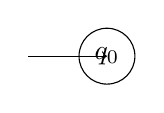
\begin{tikzpicture}
            \draw[->] (0, 0) -- (1, 0);
            
            \node[draw, circle] at (1, 0) {$q_0$} ;
        \end{tikzpicture}
        
        %\begin{figure}
        %    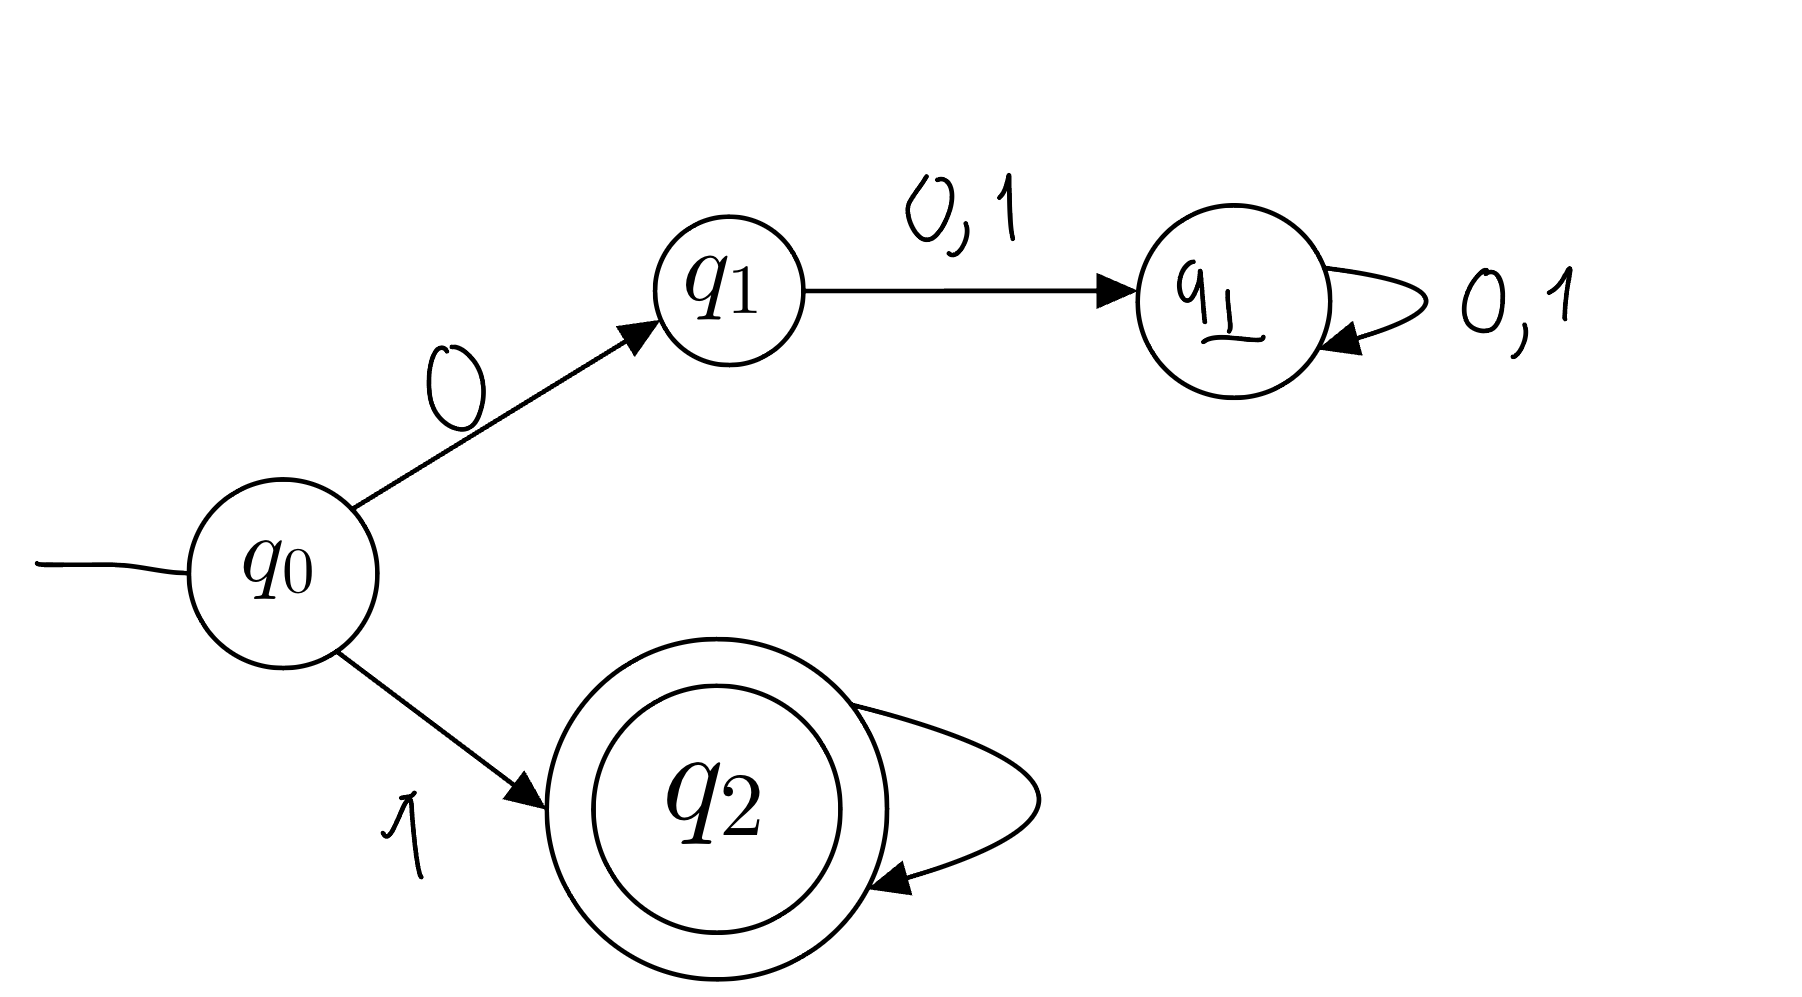
\includegraphics{Sheima/shema.png}
        %    \caption{Caption}
        %    \label{fig:my_label}
        %\end{figure}
        
    \end{example}
    \begin{definition}{chemin}{}
        Soit $\bcA = (Q,\Sigma, q_0, F, \delta)$ sur CDFA.
        
        
        Soit $v = a_1 \dots a_n  \in \Sigma^\star$ 
        
        Le chemin est dit \hg{acceptant} si $r_0 = q_0 et r_a \in F$
        On dit que $\bsA$ \hg{reconnaît} (ou \hg{accepte}) le mot $v$ s'il existe un chemin l'acceptant par v dans $\bsA$
        
    \end{definition}
    
    \begin{notation}
        \begin{enumerate}
            \itt On note $r_0\lima{a_1} r1 \lima{a_2} \dots r_{n - 1} \lima{a_n} r_n$ un chemin.
            \itt Si on ne souhaite pas spécifier tout les états intermédiaires on note $r_0 \lima{v} r_n$ lorsqu'il n'y a pas de doute sur $\bsA$.
        \end{enumerate}
    \end{notation}
    
    \begin{example}{}{}
        \begin{enumerate}
            \itt $v = 0 : q_0 \lima{0} q_1 \in F$ donc 0 est accepté par $\bsA_{bin}$.
            \itt $v = 101 : q_0 \lima{1} q_2 \lima{0} q_2 \lima{1} q_2 \in F$ Donc 101 est accepté
            \itt $v = 010 : q_0 \lima{0} q_1 \lima{1} q_\bot \lima{0} q_\bot \notin F$
        \end{enumerate}
    \end{example}
    
    On remarque que si $q \in Q$ est tel que :$\forall a \in \Sigma, \delta \p{q, a} = q$, on dit que $q$ est un état absorbant.
    
    \begin{example}{}{}
        $q_1 et q_2$ sont des états absorbants de $\bsA_{bin}$.
    \end{example}
    
    \begin{definition}{Langage d'un automate}{}
        Soit $\bsA$ un automate. Le langage de $\bsA$, noté $\bsL \p{\bsA}$, est l'ensmeble des mots acceptés par $\bsA$.
    \end{definition}
    
    \begin{example}{}{}
        $\bsL \p{\bsA_{bin}} = 0 \vert 1 \p{0 \vert 1}^\star$
    \end{example}
    
    \begin{definition}{automate déterministe incomplet}{}
        Un automae deterministe incomplet (DFA)
        est un quintuplet $\bcA = (Q,\Sigma, q_0, F, \delta)$ dont - $Q,
        \Sigma, q_0 et F$ sont definis comme pour ∞ les CDFA 
             
             - $\delta :  Q * \Sigma -> Q $ est une fonction partielle 
    \end{definition}
    
    \begin{example}{}{}
        $\bsA_{bin}'$
        
        % INSERT SHEMA n°2
        
        $\bsL \p{\bsA_{bin}'} = \bsL \p{\bsA_{bin}}$
    \end{example}
    
    
    On remarque que dans un CFDA $\bcA$, pour tout $v\in \Sigma^*$, il y a un unique chemin associé a $v$ partant de $q_0$ dans $\bcA$
    
    \begin{theorem}{completion}
        Soit $A$ = $\bcA = (Q,\Sigma, q_0, F, \delta)$ un DFA 
        il existe un unique DFA CDFA $A_c$ tel que $\bsL(A_i) = \bsL(A_c) $
        
        what do you do mean  
             
                
        
    \end{theorem}  
    
    \begin{nproof}
        On pose $\bsA_c = \ens{Q_a, \Sigma, q_0, F, \delta}$ où
        \begin{enumerate}
            \itt $Qc = Q_i \cup \ens{q_\bot}$ avec $q_\bot \notin Q_i$
            \itt $\delta_c \times \Sigma \to Q_c$ telle que :
            \begin{enumerate}
                \itt $\p{q, a} \to \delta_i \p{q, a \in dom \p{\delta_i}}$ % dom -> domaine
                \itt $(q, a) \to q_\bot si \p{q, a} \notin dom \p{\delta_i}$
                \itt $\p{q_\bot, a} \to q_\bot \forall a \in \Sigma$
            \end{enumerate}
            
        \end{enumerate}
        $q_\bot$ est appelé état pridr
        
        Montrons que $\forall v \in \Sigma^\star, v \in \bsL \p{\bsA_i} \equiv v \in \bsL \p{1_c}$
        
        $\implies$ : Si $v = q_1 \dots q_n \in \bsL \p{\bsA_i}$, alors $q_0 \lima{v}_{\bsA_i}^\star q_f \in F$. On a alors $q_0 \lima{v}_{\bsA_c}^\star q_f$, et $v$ accepté par $\bsA_c$ car :
        \begin{enumerate}
            \itt $q_0$ est l'état initial de $\bsA_c$
            \itt $F$ est l'ensemble des états finaux de $\bsA_c$
            \itt $\delta_i$ et $\delta_c$ coïncident sur deux $\p{\sigma_i}$
        \end{enumerate}
        
        
        <==
        Par contraposé: Si $v \notin \bsL(A_i) $
        \begin{enumerate}
            \itt il existe un chemin $q_0$ --------> q'. 
        
            puisque $v \not \in \bsL(A_i), q \notin F $
            
            on a donc $q_0 -------> q' \notin F $ donc $v \in \bsL(A_c)$.
            \itt si il existe pas de chemin dans $\bcA_i$ partant $q_0$ pour $v=q_1 \dots q_n$
        
        donc $\exists x \in $ [|0, n-1|] tq $u=a_1 \dots a_k$ possède un tel chemin mais pas $u_(a_k+1)$
        \end{enumerate}
        
        $q_0 = r_0 \lima{a_1} r_1 \lima{a_2} r_2 \dots \lima{a_k} r_k$ et $\p{r_k, a_{k+1}} \notin dom \p{\delta_i}$
        on a donc le chemin
        $q_0 = r_0 \lima{a_1} r_1 \lima{a_2} r_2 \dots \lima{a_k} r_k \lima{a_{k+1}} q_\bot \dots \lima{a_n} q_\bot \notin F$
            
        
        Donc $v \notin \bsL(A_c)$
    \end{nproof}
    
    
    
    \begin{example}{}{}
        $\bcA_bin$ est le completé de $\bcA_bin'$
        par se prossesus 
        
    \end{example}
    
    \begin{definition}{etat accesible}{}
        Soit $\bsA = \ens{Q, \Sigma, q_0, F, \delta}$ un DFA.
        Un état $q \in Q$ est dit \hg{accessible} si $\exists v \in \Sigma^\star$ tel que $q_0 \lima{v}_\bsA^\star q$
    \end{definition}
    
    On remarque que pour trouver l'ensemble des "tats accessibles, il suffit de faire un parcours de graphe en partant de $q_0$.
    
    \begin{definition}{etat coaccessible}{}
        
        Soit $\bsA_c = \ens{Q_a, \Sigma, q_0, F, \delta}$ un DFA.
        
        Un etat $q\in Q$ est dit co-accesible si 
        
        $\exists v \in \Sigma^*$, $\exists q_f \in F $ tq $ q \lima{v *}{\bsA} q_f$
        
    \end{definition}
    
    On remarque que pour trouver l'ensemble des état co-accessible, on peut faire un parcours de graphe en partant des états $q_f \in F $ et on remantant les arcs.
    
    \begin{example}{}{}
        % INSERT SHEMA 3 HERE
        \begin{enumerate}
            \itt $q_0$ et $q_1$ sont co-accessibles
            \itt $q_2, q_3, q_4$ ne sont pas co-accessibles
        \end{enumerate}
    \end{example}
    
    
    \begin{definition}{état utile}
        Soit $\bsA = \ens{Q, \Sigma, q_0, F, \delta}$ un automate
        Un état $q \in Q$ est dit utile s'il est a la fois accessible est co-accessible 
        
    \end{definition}
    \begin{definition}{émondé}{}
        Un automate est dis émondé si tous ces état ces état sont utiles 
    \end{definition}
    On remarque que émondé n'implique pas qu'il soit le plus petit possible  
    
    \begin{example}{}{}
        DESSIN de rayan "sheima 3"  
        %
        $\bcA$ et $\bcA'$ sont émondés et $\bcL\p{\bcA} = \ens{a, b}^\star = \bcL\p{A'}$.
    \end{example}
    %MAIS ECRIT JUSTE N'IMPLIQUE PAS MDR
    %non mdrrrrrrr je veux faire des symbolle 
    
    \subsection{Automates non déterministes}
    
    \begin{definition}{Automate fini non déterministe}
        On appelle automate fini non déterministe (NFA) un quintuplet $\bcA = \p{Q, \Sigma, q_0, F, \delta}$ où :
        %
        \begin{enumerate}
            \itast $Q$, $\Sigma$, $q_0$, $F$ sont définis comme pour les DFA ;
            
            \itast $\delta : Q \times \Sigma \to P\p{Q}$ est une fonction partielle appelée \hg{relation de transition}.
        \end{enumerate}
    \end{definition}

    \begin{definition}{Chemin}{}
        Soit $\bsA = \ens{Q, \Sigma, q_0, F, \delta}$ un NFA 
        Soit $v = a_1 \dots a_n \in \Sigma^\star$.
        
        Un chemin dans $\bcA$ pour $v$ est une séquence de $n+1$ états $r_0, r_1, \dots, r_n$ tels que :
        
        \begin{enumerate}
            \itast $\forall i \in \iint{0, n}$, $r_i \in Q$.
            
            \itast $\forall i \in \iint{1, n}, r_i \in \delta\p{r_{i-1}, a_i}$.
        \end{enumerate}
    
    le chemin est dis acceptant si $r_0=q$ et $r_n \in F$.
    Un mot $v$  est accepté par $\bcA$ si $\exists$ un chemin acceptant pour $v$ dans $\bcA$ . 
    
    
    
    
    %pourquoi qaund j'ecris "B S" ca remplace auto par Brawl Stars 
    %???????????????????????
    
    
    \end{definition}
    
    \begin{example}{}{}
        $\bcA_{a3} :$
        %
        Dessin %ok je fais le sheima 4 et je garde sheima 
        %
        \begin{enumerate}
            \item 
            
            
            \itt $abaa \notin \bsL(\bcA_{a3})$
        \end{enumerate}
    \end{example}
    %mdrrrrr y a un stack d'erreur 
    
    
    remarque: Pour tester si $v\in \bsL\p{bsA} a$ avec $\bsA$ un NFA, il faut "deviner" le chemin qui va être acceptant : il faut a priori tous les tester jusqu'a ce qu'il y en ai un qui marche. On peut utiliser le backtracking.
    
    \begin{definition}{}{}
        Un automates finis (non déterministe) 
        à transition spontanné ($\varepsilon -$NFA) %NFA comme nouveau pere fondateur 
        est un quintuplet $\bsA = \ens{Q, \Sigma, q_0, F, \delta}$ ou 
        
        \begin{enumerate}
            \itt $Q, \Sigma, q_0, F$ sont définis comme pour les NFA
            \itt $\delta Q x \p{\Sigma \cup \ens{\epsilon}} \to \bsP \p{Q}$ est une fonction partielle
        \end{enumerate}
        
    \end{definition}
    
    On remarque que dans $v_n$ les $\varepsilon$ - NFA,  les transitions de la forme $q \lima{\epsilon} q'$ sont appelées des transitions spontanées (ou $\epsilon$ transition).
    
    
    \begin{definition}{chemin}{}
        Soit $\bsA = \p{Q, \Sigma, q_0, F, \delta} un \epsilon-NFA$ Soit $v \in \Sigma^\star$ Un chemin dans $\bsA$ pour v est une séquence finie $r_0, \dots , r_n$ de $n+1$ états tq :
        
        \begin{enumerate}
            \itt $\exists (a_1, \dots, a_n) \in \p{\Sigma \cup \ens{\epsilon}}^n tq v = a_1 \dots a_n$
            \itt $\forall i \in \iint{0, n}, r_i \in Q$
            \itt $\forall i \in \iint{1, n}, r_i \in \delta \p{r_{i-1}, a_i}$
        \end{enumerate}
            
    \end{definition}
    
    \begin{example}
            dessin 5 sur le discord
            %je fais le schema 5
            
            \begin{enumerate}
                \itt $\epsilon \in \bsL \p{\bsA}$
                \itt $ac \in \bsL \p{\bsA}$
                \itt $bbbb \in \bsL \p{\bsA}$
            \end{enumerate}
        $\bsL \p{\bsA} = \p{a \enstq b}^\star b^\star c^\star$
        $ = \p{a \enstq b}^\star c^\star$
    \end{example}{}
    
    \subsection{Déterminisation, suppression des $\varepsilon$-transitions}
    
    Nous avons introduit 3 modèles d'automates: les DFA, les NFA, et les $\epsilon$-NFA. Nous allons maintenant montrer que ces 3 modèles sont équivalents.
    
    %%go pour une preuve qui fais 3 tableaux avec 50 schema 
    
    
    \begin{definition}
        Soit $\bcA_N = \ens{Q_N, \Sigma, q_0, F_N, \delta_N }$ un NFA
        
        
        On appelle automates des parties de $\bcA_N$, noté $\det(\bcA_n)$
        l'automate déterministe $\bcA_D = \ens{Q_D, \Sigma, \ens{q_0}, F, \delta_D}$ tel que :
        %
        \begin{enumerate}
            \itast $Q_D = P\p{Q_N}$
            
            \itast $F_D = \ens{S \enstq S \subseteq Q_N, S \cap F_N \neq \emptyset }$
            
            \itast $\delta_D : \begin{array}[t]{rcl}
                Q_D \times \Sigma &\to& Q_D  \\
                \p{S, a} &\mapsto& \displaystyle\bigcup_{q \in S} \delta_N\p{q, a} 
            \end{array}$
        \end{enumerate}
        
        
    \end{definition}
    
    \begin{example}{}{}
            %j'ai pris une photo et je l'ai giga compresser 
        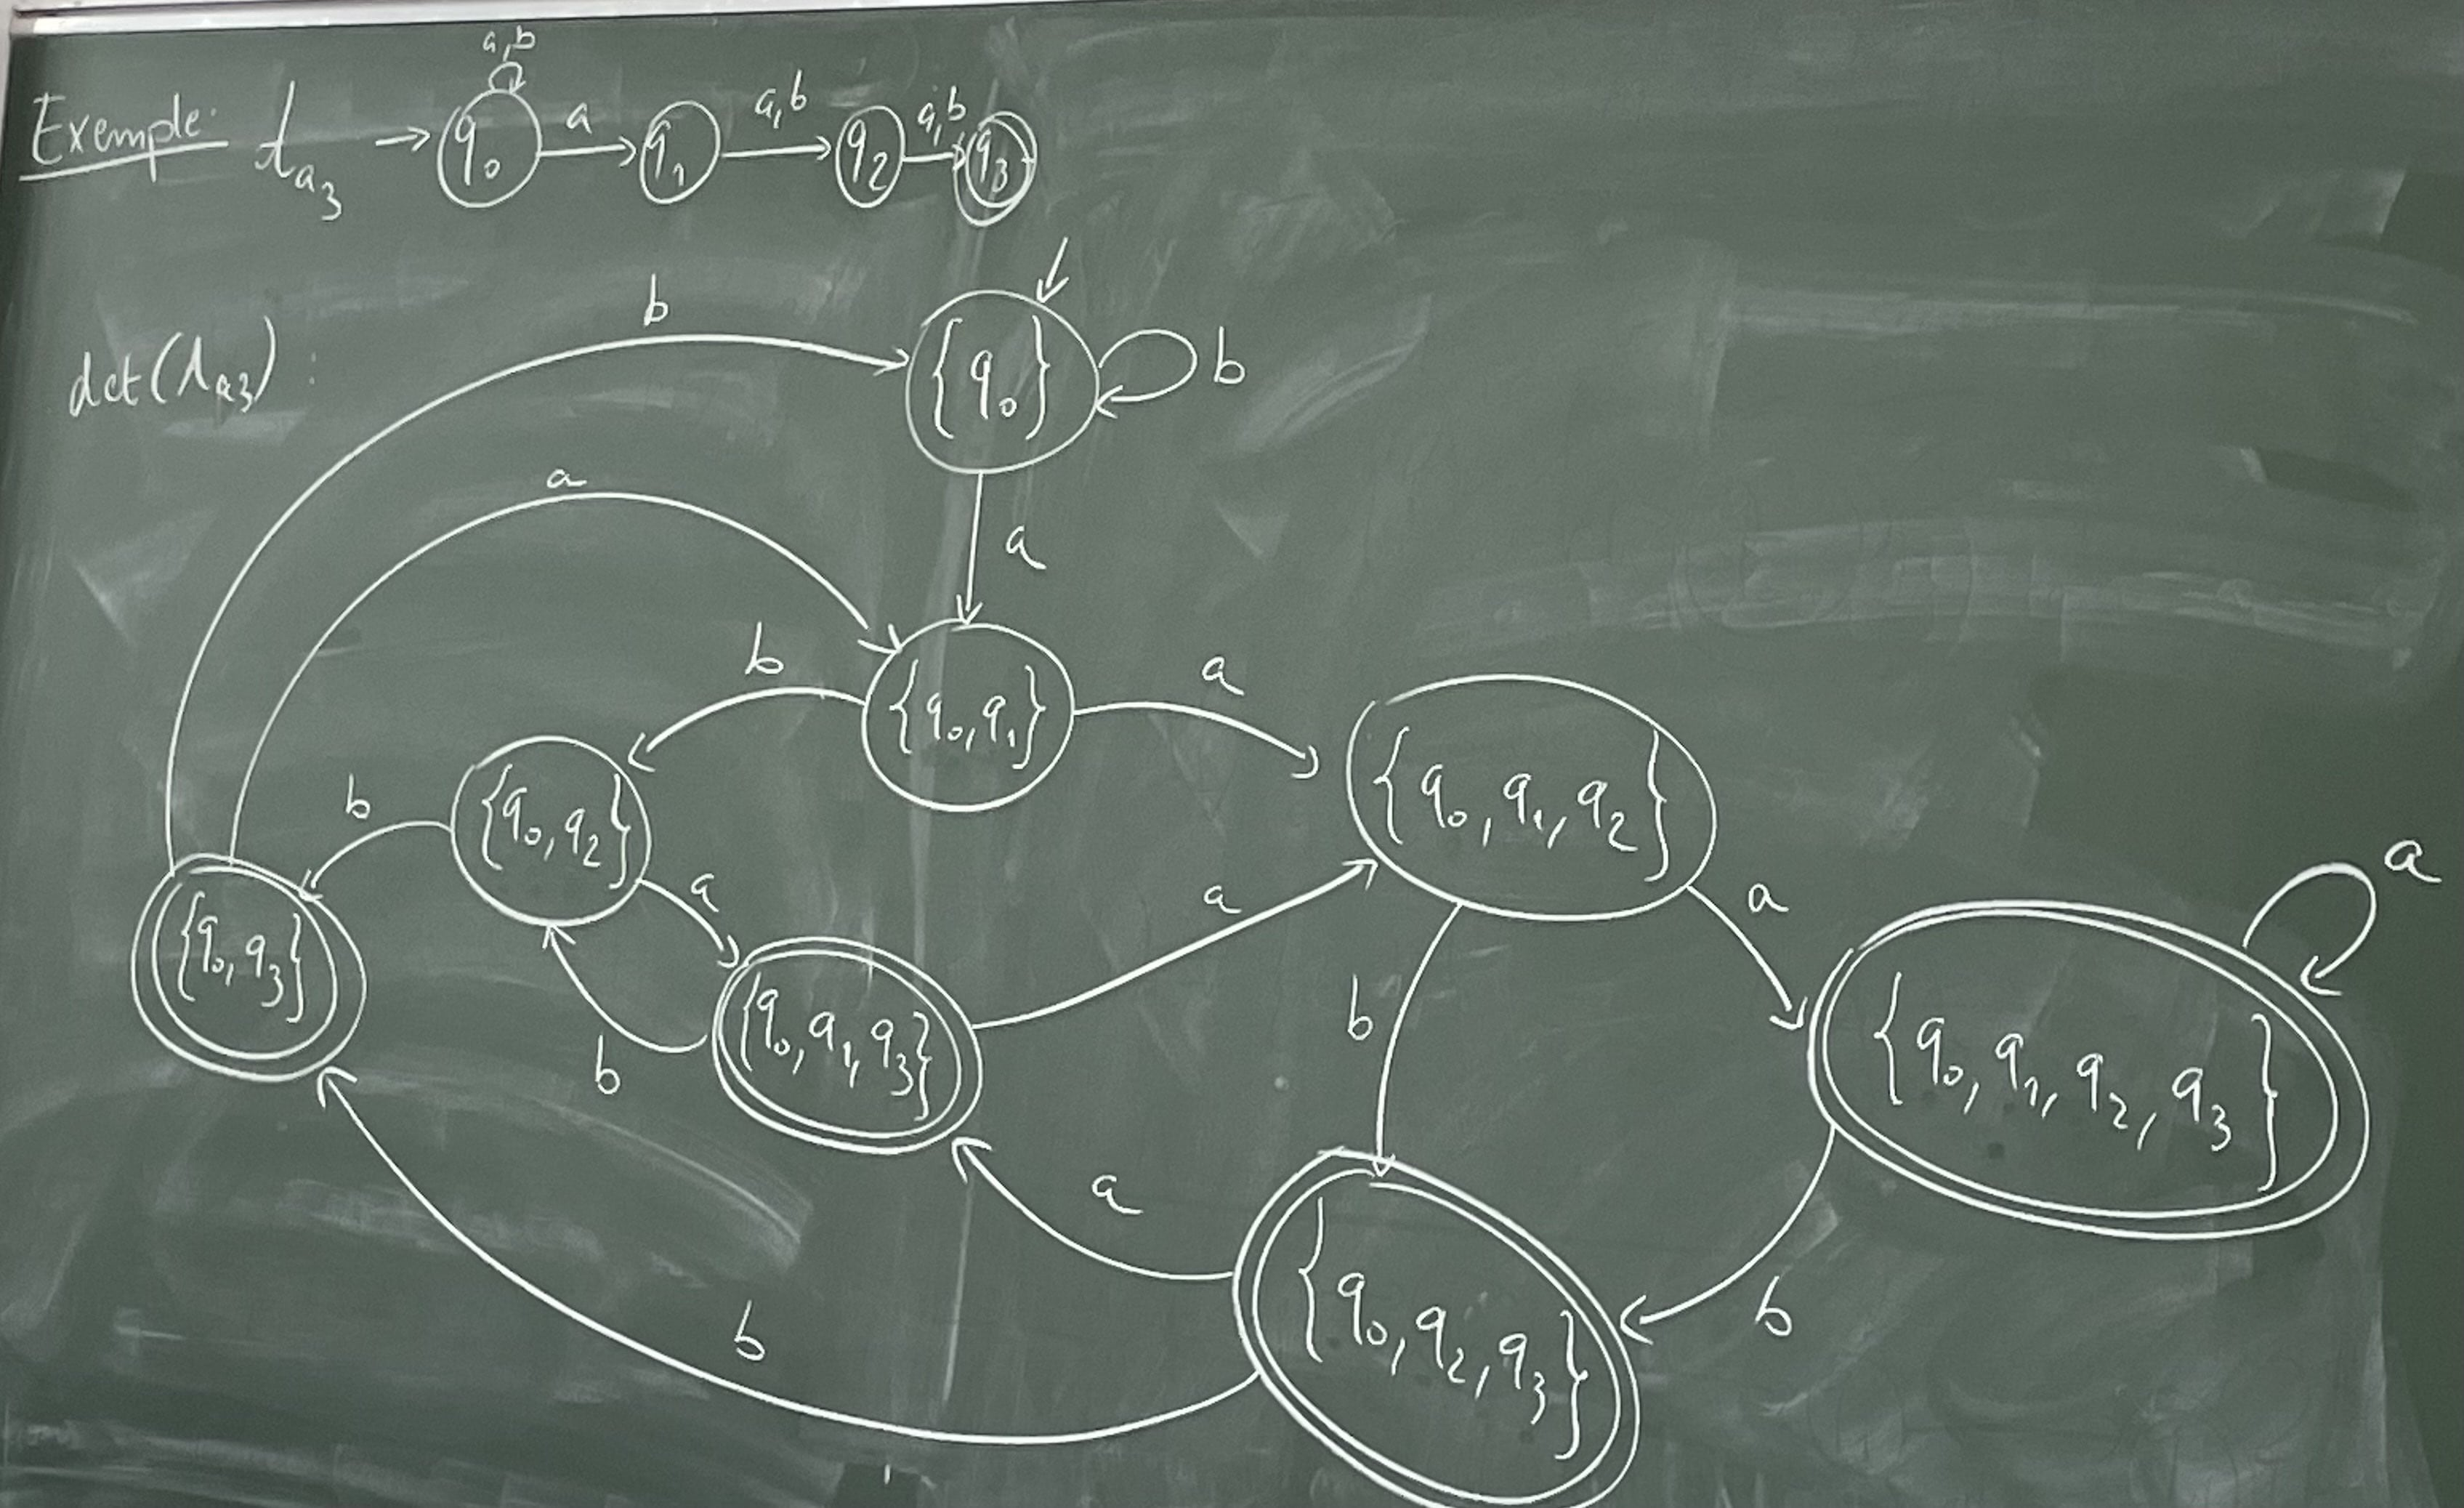
\includegraphics[scale=0.1]{Sheima/grosse_sheima.jpeg}
    \end{example}
    
    \begin{theorem}{}{}
        Soit $\bcA_N = \p{Q_N, \Sigma, q_0, F_n, \delta_n}$ un NFA.
        On a $\bcL\p{\bcA_n} = \bcL\p{\det\p{\bcA_n}}$
    \end{theorem}
    
    \begin{nproof}
        Montrons que $\forall v \in \Sigma^\star$ et $r_0 \to r_1 \to \dots \to r_n$ l'unique chemin dans $\det \p{\bsA_n}$ pour $v$ (avec $R_0 = \ens{q_0}$), on a $R_n = \ens{q \in Q_n \enstq \exists q_0 \lima{v}{\bsA_n^\star} q}$.
        
        Par récurrence sur $\mod{v}$ :
        %
        \begin{enumerate}
            \itt si $\mod{v} = 0 : v = \epsilon$ donc $R_0 = \ens{q_0}$, alors c'est bon.
            
            \itt $\mod{v} = n + 1$ : Supposons la propriété vraie pour tout mot de taille $n$ Montrons qu'elle est vraie pour $v$ :
            
            $v = ua$ avec $\mod{u} = n$ et $a \in \Sigma$.
            
            Soit $R_0 \lima{u} {}^\star R_n \lima{a}{} R_n+1$ dans $ \det{\bsA_n}$.
            
            Par hypothèse de récurrence, $R_n = \ens{q \in Q_n \enstq \exists q_0 \lima{u}{\bsA_n^\star} q}$
            
            Par définition de $\delta_\bsD$ :
            $R_{n+1} = \delta_\bsD \p{R_n, a} = \bigcup_{q \in R_n} \delta_n \p{q, a} = \ens{q' \ in Q_n \enstq \exists \lima{v}{\bsA_n}^\star q'}$
            
            \itt On a fait toutes les positions des chemins : $q_0 \lima{u}{\bsA_n}^\star q'$
        
        
        
            Par définition de $F_d$
            
            \begin{align*}
                v \in \bcL\p{\det{A_n}} &&\iff&& \ens{q_0} \lima{v^\star} R_n &&\text{avec} \ R_n \cap F_n \neq \emptyset\\
                &&\iff&& \exists q_0 \lima{v}^\star_{\bcA_n} q &&\text{avec} q \in F_n
            \end{align*}
            
        \end{enumerate}
    \end{nproof}
    
    \begin{corollary}{}{}
        Soit $L \subseteq \Sigma^\star$ un langage : L est reconnaissable par un DFA si et seulement si L est reconnaissable par un NFA.
    \end{corollary}
    
    \begin{nproof}
        ($\Leftarrow$<=) Si $L = \bsL \p{\bsA_n}$ avec $\bsA_n$ DFA alors $L = \bsL \p{\bsA_\bsD}$ avec $\bsA_\bsD = det \p{\bsA_n}$
        ($\rightarrow$=>) Si $\bsA_\bsD = \p{Q, \Sigma, q_0, F, \delta_\bsD}$ un DFA tq $L = \bsL \p{\bsA_\bsD}$
        Alors$\bsA_n = \p{Q, \Sigma, q_0, F, \delta_n}$ avec $\delta_n \p{q, a} = \ens{\delta_\bsD \p{q, a}}$ pour tout $q \in \alpha, a \in \Sigma$ vérifie $L \in \bsL \p{\bsA_n}$
    \end{nproof}
    
    On va maintenant montrer comment supprimer les $\epsilon$-transitions.
    
    \begin{definition}{$\epsilon$-fermeture}{}
        Soit $\bsA = \ens{Q, \Sigma, q_0, F, \delta}$ un $\epsilon$-NFA. 
        Soit $q\in Q $ %une ligne
        
        on appelle $\varepsilon$-fermeture de q l'ensemble: 
        
        %remy a supprimer la formule
        
    \end{definition}
    \begin{notation}
        Si $Q' \subseteq \text{  , } E(Q') = \bigcup E(q) $ %greve de deux tableau 
        
    \end{notation}
    
    %manque 1 definition, 1 notation, 1 theoreme, 1 corrolaire, 1 definition 
    
    \section{Theoreme de Kleeme}
    
    \begin{theorem}{de Kleeme}{}
    Soit $\Sigma$ un alphabet 
    
    
    $Rcc_\Sigma = Reg_\Sigma$
    
    %gros paragraphe 
    \end{theorem}
    \begin{definition}{automates de Thomposon}{}
        
    \end{definition}
    
    \begin{nproof}{Par induction}
        plein de petite sheima par millier 
        
    \end{nproof}
    
    On remarquera que dans les automates de \textsc{Thompson}, on a souvent la situation suivante :
    %
    \begin{tikzpicture}
        
    \end{tikzpicture}
    %
    En réalité, les \guill{vrais} états initiaux sont $q_{i_1}, \dots, q_{i_n}$ mais notre définitions des automates impose d'avoir un seul état initial. Dans la définitions des NFA, on peut en fait autoriser un ensemble $I \subseteq Q$ d'états initiaux au lieu d'un unique $q_0$. Dans ce cas, pour l'automate des parties (algorithme pour déterminer un NFA), il faut choisir $I$ à la place de $\ens{q_0}$ pour l'état initial.
    
    \begin{theorem}{}{}
        Soient \hg{$\Sigma$ un alphabet} et \hg{$r$ une expression régulière} sur $\Sigma$. On a :
        %
        \[ \hg{\bcL\p{\th r} = \bcL\p{r}}\]
    \end{theorem}
    
    \begin{nproof}
        Soient $\Sigma$ un alphabet et $r$ une expression régulière sur $\Sigma$. On procède par induction structurelle sur $r$. Traitons d'abord les cas de base :
        %
        \begin{enumerate}
            \itt Si $r = \emptyset$, on a $\th r = \th \emptyset = $ dessin.
            
            Dans ce cas, $\bcL\p{\th r}\bcL\p{\th \emptyset} = \emptyset = \bcL\p{\emptyset} = \bcL\p{r}$.
            
            \itt Si $r = \epsilon$, on a $\th r = \th \epsilon = $ dessin.
            
            Dans ce cas, $\bcL\p{\th r} = \bcL \p{\th \epsilon} = \ens{\epsilon} = \bcL\p{\epsilon} = \bcL\p{r}$
            
            \itt Si $r = a$, on a $\th r = \th a = $ dessin.
            
            Dans ce cas, $\bcL\p{\th r} = \bcL \p{\th a} = \ens{a} = \bcL\p{a} = \bcL\p{r}$
        \end{enumerate}
        %
        Pour l'induction, on considère $r_1$ et $r_2$ deux expressions régulières telles que :
        %
        \[ \bcL\p{\th r_1} = \bcL\p{r_1} \qquad\et\qquad \bcL\p{\th r_2} = \bcL\p{r_2} \]
        %
        On pose $A_1 = \th r_1$ et $A_2 = \th r_2$. Traitons alors les différentes règles d'induction, en considérant un $r$ obtenu à partir de $r_1$ et $r_2$. On pose directement $A = \th r$. On a :
        %
        \begin{enumerate}
            \itt Si $r = r_1r_2$, alors :
            %
            \[ A :\quad \to q_1 \lima{\epsilon} q_i^1 A_1 q_f^1 \lima{\epsilon} q_i^2 A_2 q_f^2 \lima{\epsilon} q_f\]
            %
            Soit $v \in \bcL\p{r_1r_2}$, alors il existe $v_1 \in \bcL\p{r_1}$ et $v_2 \in \bcL\p{r_2}$. Par hypothèse, on a donc $v_1 \in \bcL\p{A_1}$ et $v_2 \in \bcL\p{A_2}$.
            
            Puisque $v_1 \in \bcL\p{A_1}$, il existe un chemin $q_i^1 \lima{v_1}_{A_1}^\star q_f^1$.
            
            De même, $v_2 \in \bcL\p{A_2}$, il existe un chemin $q_i^2 \lima{v_2}_{A_2}^\star q_f^2$.
            
            Donc :
            %
            \[ q_i \lima{\epsilon} q_i^1 \lima{v_1}{}_A^\star q_f^1 \lima{\epsilon}  q_i^2 \lima{v_2}{}_A^\star q_f^2 \lima{\epsilon}  q_f\]
            %
            Donc $\epsilon v_1 \epsilon v_2 \epsilon \in \bsL \p{A}$
        (car $\epsilon v_1 \epsilon v_2 \epsilon = v_1 v_2 = v$)
        ainsi $\bsL\p{r_1r_2} \subseteq \bsL(A)$ 
            
        
        Réciproquement, si $v\in \bsL(\bcA)$, forcément le chemin acceptant $v$ dans $\bcA$ est de la forme précédente, donc $v= \epsilon v_1 \epsilon v_2  \epsilon $
        
        
        Donc $v = v_1v_2$ avec $v_1 \in \bcL\p{A_1} = \bcL\p{r_1}$ et $v_2 \in \bcL\p{A_2} = \bcL\p{r_2}$ d'où $v \in \bcL\p{r_1r_2}$, ainsi $\bcL\p{A} \subseteq \bcL\p{r_1r_2} = \bcL\p{r}$.
        
            \itt Si $r = r_1 \vert r_2$, alors :
            
            \textcolor{magenta}{DESSIN}
            
            Soit $v \in \bcL\p{r_1 \vert r_2}$. Par hypothèse d'induction, on a $v \in \bcL\p{A_1}$ donc $q_i^1 \lima{v}_{A_1}^\star q_f^1$. Par construction, 
            %
            \[ q_i \lima{\epsilon} q_i^1 \lima{v}_A^\star q_1^f \lima{\epsilon} q_f\]
            %
            accepte $v$ dans $A$, donc $v \in \bcL\p{A}$, d'où $\bcl\p{r_1 \vert r_2} \subseteq \bcL\p{\bcA} = \bcL\p{\th r}$.
            
            Réciproquement, si $v \in \bcL\p{A}$, alors son chemin acceptant est de la forme :
            %
            \[ q_i \lima{\epsilon} q_i^1 \lima{v}_{A}^\star q_f^1 \lima{\epsilon} q_f \qquad\ou\qquad TODO\]
            %
            Donc $v \in \bcL\p{A_1}$ ou $v \in \bcL\p{A_2}$. Par hyptohèse d'induction, $v \in \bcL\p{r_1} \cup \bcL\p{r_2} = \bcL\p{r_1 \vert r_2}$.
            
            \itt Si $r = r_1^\star$, alors :
            %
            \textcolor{magenta}{\Huge{DESSIN}}
            %
            Soit $v \in \bcL\p{r_1^\star} = \bcL\p{r_1}^\star$. Il existe un entier $m \in \bcN$ tel que $v = v_1 \dots v_m$ avec $v_i \in \bcL\p{r_1}$ pour $i \in \iint{1, m}$.
            
            Montrons par récurrence sur m que $v \in \bsL \p{A}$ :
            \begin{enumerate}
                \ithand Si $m = 0$, alors $v = \epsilon \in \bsL \p{A}$ car $q_i \lima{\epsilon} q_i^1 \lima{\epsilon} q_f^1 \lima{\epsilon}  q_f$
                    
                \ithand Si $m \geq 1$, alors par hypothèse de récurrence, $v_1\cdots v_{n+1} \in \bcL\p{A}$. Donc :
                %
                \[ q_i \lima{\epsilon} q_i^1 \lima{v_1\dots v_{n-1}}_A^\star q_f^1 \lima{\epsilon} q_f\]
                %
                Or $v_m \in \bcL\p{r_1} = \bcL\p{A_1}$ soit l'hypothèse de récurrence. Ainsi $q_i^1 \lima{v_m}_{A_1}^\star q_f^1$.
            \end{enumerate}
                
            Donc $v$ est accepté dans $A$ par:    
            %
            \[ q_i \lima{\epsilon} q_i^1 \lima{v_1 \dots v_{m-1}}_A^\star q_f^1 \lima{\epsilon} q_i^1 \lima{v_m}_A^\star q_f^1 \lima{\epsilon} q_f \]
            %
            Donc $v \in \bcL\p{A}$. Réciproquement, soient $v \in \bcL\p{A}$ et $q_i \lima{v}_A^\star q_f$ acceptant $v$.
            %
            \begin{enumerate}
                \ithand Si $q_i \lima{\epsilon} q_i^1 \lima{\epsilon} q_f^1 \lima{\epsilon} q_f$, alors 
                
                \ithand 
                
                \ithand sinon, on peut toujours se ramener à un chemin n'ayant pas de morceau de la forme :
                %
                \[ q_i \lima{\epsilon} q_i^1 \lima{v_1}_{A_1}^\star q_f^1 \lima{\epsilon} q_i^1 \lima{v_2}_{A_1}^\star \lima{\epsilon} q_i^1 \lima \dots \lima{v_m}ç{A_1}^\star q_f^1 \lima{\epsilon} q_f\]
                %
                Donc $v =v_1 \dots v_m$ avec $v_i \in \bcL\p{A_1} = \bcL\p{r_1}$ pour $i \in \iint{1, m}$, donc $v \in \bcL\p{r_1^\star}$.
             \end{enumerate}
        \end{enumerate}
    \end{nproof}
    
    On remarquera que cette preuve est constructive. Elle fournit donc un algorithme qui, à partir d'une expression régulière $r$, fournit un automate reconnaissant $\bcL\p{r}$. L'automate de \textsc{Thompson} doit son nom à l'informaticien \textsc{Ken Thompson} qui a créé l'outil \texttt{grep}, reposant sur la construction des automates (de \textsc{Thompson}). 
    
    On remarquera par ailleurs que 'l'on vient de montrer que $\mathrm{Reg}_\Sigma \subset \mathrm{Rec}_\Sigma$. La section suivante propose une autre démonstration (elle aussi constructive) de cette inclusion.
    
    \subsection{Algorithme de Berry-Sethi, automate de Glushkov}
        
    \begin{definition}{Langage local}{}
        Soit $\Sigma$ un alphabet, et $L \subset \Sigma^\star$ un langage. On note :
        %
        \begin{enumerate}
            \itast $\First\p{L} = \ens{a \in \Sigma \enstq \ens{a}\Sigma^\star \cap L \neq \emptyset}$
            
            \itast $\Last\p{L} = \ens{a \in \Sigma \enstq \Sigma^\star\ens{a} \cap L \neq \emptyset}$
            
            \itast FACTS
            
            \itast NFACTS
        \end{enumerate}
    \end{definition}
    
    \begin{example}
            exemple triviale 
            
            
            
            Soit $v \in (First(L1)\Sigma $ %remy ecrit %LOL NON TA CRU
            
            
    \end{example}
    
    \begin{definition}{automate de Glushkov}{}
        Soit $\Sigma$ un alphabet et $L \subset \Sigma^\star$ un langage local. On appelle \hg{automate de \textsc{Glushkov}} de $L$ l'automate $\Loc{L} = \p{Q_L, \Sigma, q_0, F_L, \delta_L}$ tel que :
        %
        \begin{enumerate}
            \itast $Q_L = \ens{q_0} \cup \ens{q_a \enstq a \in \Sigma}$
            
            \itast $F_L = \ens{q_a \enstq a \in \Last{L}} $
        \end{enumerate}
        
        
    \end{definition}
    
    \begin{theorem}
        Soit $\Sigma$ un alphabet et $L \subseteq \Sigma^\star$ un langage local. $L = \bcL(Loc(L))$
    \end{theorem}
    \begin{nproof}
        L $\subset \bsL(Loc(L))$
        \begin{enumerate}
            \itt \Huge{blablablablbalbal}
        \end{enumerate}
    \end{nproof}
        
        
    
    
    